\section{Our Approach}
\label{s:solution}

Our solution integrates three contributions to address these requirements:
\begin{enumerate}
\item An RDF vocabulary for describing log and monitoring data collections
      in terms of the subject being monitored, the time period covered,
      the type and format of the data and details for accessing the data or
      contacting its curator.
      
      The defining characteristic of a \texttt{ConcreteLog} - that is, a 
      specific file/stream/block-of-data being described - in the vocabulary
      is that it has a \emph{subject} - ie what the log reports on - and 
      that its entries have associated temporal information. This is a 
      sufficiently broad definition to cover all log-like collections
      while providing dimensions for a search to operate in.
      
\item A schema for publishing annotations, linked to log data, in an SQL
	  database. Annotations might be:
      
\begin{itemize}
\item Expert commentary, such as ``this log message means that down links
      caused the network to be quiesced while re-calculating routing tables''      
\item Human observations, such as ``during this period our engineer was 
      replacing some failed nodes, so the network was probably disrupted'' 
\item Machine-generated observations, such as message-pattern frequencies 
      computed by running certain logs through an analysis tool such as 
      Baler\textcolor{red}{cite}.
\end{itemize}

      The schema includes fields for the  components and the time period to 
      which each annotation applies, allowing annotation sets to also be 
      described with the RDF vocabulary

\item A collection of tools to make the RDF vocabulary and annotation 
      schema accessible to users, system administrators and support staff.

      While nothing prevents annotators and researchers from directly 
      annotating, describing and querying collections with SQL and RDF, 
      the learning curve for these technologies presents an entry 
      barrier to the time-constrained individuals who would otherwise
      benefit from it. 
      
      Many interactions with annotated, discoverable log data can be 
      can be described in just a few use cases:
      
\begin{itemize}
\item Cataloging a collection to make it discoverable
\item Annotating specific logs, either to add expert commentary to 
      entries of interest or to associate human observations with log 
      entries, log subjects or time periods
\item Finding data relevant to a subject and time period of interest
\item Extracting slices of logs associated with specific annotations, 
      or periods and subjects of interest
\end{itemize}

     The diversity of data sources and formats mean that these use cases 
     can be extended almost indefinitely, and providing a generalized 
     interface to every conceivable HPC component and data format is 
     not the goal here (see philosophy point \textcolor{red}{X}). We 
     do, however, provide an extensible tooling infrastructure and tools
     for some basic and common scenarios.

\end{enumerate}

\subsection{RDF Vocabulary}

The need for a decentralized mechanism for publishing information whose 
\emph{meaning} is machine-readable has been known for more than two decades
\textcolor{red}{cite https://www.w3.org/Talks/WWW94Tim/}. Since then a 
collection of tools and technologies supporting this has accumulated, with
perhaps the most significant being the specification of RDF as a data 
interchange format for the World Wide Web. \textcolor{red}{cite https://www.w3.org/RDF/?}
In RDF \emph{things} (concepts or concrete items) are represented as URIs
and arranged in \emph{triples} of a \emph{subject}, a \emph{predicate} and 
an \emph{object}. 

% do this as a figure, see Ann's example
\begin{figure*}
\begin{minted}{turtle}
@prefix nersc: <http://portal.nersc.gov/project/mpccc/sleak/nersc#> .
@prefix rdfs: <http://www.w3.org/2000/01/rdf-schema#> .
@prefix foaf: <http://xmlns.com/foaf/0.1/> .
nersc:nersc rdfs:type foaf:Organization .
\end{minted}

\caption{A triple of (subject, predicate, object) describes an edge 
in an RDF graph. The \texttt{Turtle}\textcolor{red}{cite} syntax shown
here aids human readability by condensing URIs into a prefix and a suffix,
so \texttt{rdfs:type} expands as
\texttt{<http://www.w3.org/2000/01/rdf-schema\#type>}.}
\label{f:rdftriples}
\end{figure*}

For example, in Figure~\ref{f:rdftriples} the subject is a URI that 
we've chosen to associate with NERSC. In reality, this is a web address where we can 
(TODO make this more readable)
the URI up to the final ``/'' is a web address the authors
can publish files from, where we have added an RDF file called ``nersc.ttl'' 
which includes an entry also called ``nersc''. If you point a web browser 
there you will see a ``404'' error because the ``.ttl'' suffix is missing 
(other public namespaces solve this with HTTP content negotiation) - but the 
point is, we are confident that this is a unique URI we can use as an 
identifier for NERSC. (And if a better identifier for NERSC comes along 
we can link the two, also with RDF).

The predicate here is one predefined by the RDF Schema to indicate the ``type''
of a thing.

And the object is a URI predefined by the Friend-of-a-friend ontology to
indicate an Organization.

A collection of triples forms a graph whose edges have well-defined meanings, 
allowing information about nodes to be inferred from their relationships to 
other nodes.

Crucially, an RDF graph can be queried using SPARQL \textcolor{red}{cite}, a
graph-query language with a look-and-feel based on SQL. A SPARQL query 
arranges variables into a set of triples and returns sets of URIs for which
the triples for a true statement. For example, the following SPARQL query
will return the name and the web page for each node whose type is 
a subclass of \texttt{foaf:Agent}. \texttt{foaf:Agent} is a superclass for a Person, a 
Group or an Organization, so this query in English is ``list the name and 
webpage for each Person, Group or Organization in this graph''. (The 
\texttt{rdfs:subClassOf*} syntax indicates that the query should follow 
\texttt{rdfs:subClassOf} edges to any depth until a \texttt{foaf:Agent} is encountered)

\begin{minted}{sparql}
SELECT ?name ?page 
WHERE {
    ?uri a ?type .
    ?type rdfs:subClassOf* foaf:Agent .
    ?uri foaf:name ?name .
    ?uri foaf:page ?page .
}
\end{minted}

\textcolor{red}{TODO: draw this as a diagram, probably explains it better}
\textcolor{red}{TODO: prob need a ref to an "intro to semantic web" resource}

\subsubsection{Why RDF?}

-- next: why is RDF useful for solving our problem

\subsubsection{The vocabulary}

\textcolor{red}{TODO include a diagram}


-- some key things to call out:
\begin{itemize}
\item someone publishing a logset doesn't need to know many people to get their 
      logset into the graph - a curator of their local (site) catalog is enough. 
      That curator then knows curators of at least one other catalog and thus 
      gets the local 
      subgraph into the global graph
\item someone using the graph doesn't need to know who published what - they can
      query the graph itself and get metadata about what is out there, including contact 
      information for data they don't directly have access to. This allows them to 
      solve specific access limitations in a locally-appropriate way
\end{itemize}

 
\subsection{Annotation Schema}

In this subsection we describe the major fields necessary to support the
architectural requirements that pertain to the annotations themselves
(as opposed to the remote discovery infrastructure). The prototype
implementation is an SQLite database, so we descirbe in in terms
of that implemention, however that is not required. More generally
this would be descirbed in terms of accessor APIs independent of
the implementation beneath them.

The annotations table is defined as:
\begin{small}
\begin{minted}{sql}
CREATE TABLE 'annotations' (
       'id' integer,
       'authorid' char(3) NOT NULL,
       'starttime' datetime NOT NULL,
       'endtime' datetime NOT NULL,
       'startstate' text,
       'endstate' text,
       'description' text NOT NULL,
       'manual' boolean,
       'logfiles' text,
       'system' text,
       'systemdown' boolean,
       'LDcatgroup' text \
          REFERENCES 'LDgroups'('id'),
       'LDcategory' text,
       'LDtag' text,
       'components' text,
        balerpatternid integer,
        PRIMARY KEY('id','authorid')
        );
\end{minted}
\end{small}

The major fields for an annotations include \texttt{description}, \texttt{starttime}, \texttt{end time},
\texttt{system}, and \texttt{components} involved.
The description is a descriptive translation of a log messge or event (Examples
are given in Section~\ref{s:annotations}); it is this description to which we
mainly refer when we refer to an annotation.
The \texttt{authorid} identifies the author of an annotation, who
is responsible for the determination of the content of the assignable fields
(such as the description); the authorid and annotation id together form a unique key.
Time and component fields refer to a specific instance of a log line or event
occurence. Thus multiple annotated log line instances may share the same description,
but have different time and component values.

Other information is used to help with context and search.
For example, \texttt{startstate} and \texttt{endstate}, which
are subjective and can be used to record things like a component
that starts a faulty but is repaired by the action of the annotations,
for example, if the event is recording that a DIMM was changed.
\texttt{Systemdown} is meant to aid in the search for events that result
in full system failure.

\texttt{Manual} is used to indicate manually performed
events, such as an administrator action to take down a node as opposed
to the system taking down a node because it failed a health check.
Knowledge of this can be used to more accurately determine the
number of true failure events and for assessing the effectiveness
and availability of system resilience mechansims vs required
human intervention.

A set of fields, \texttt{LDXXX} are available to give contextual inforatmion.
At the moment only \texttt{LDcategory} is used; this is used to define the major
subsystem relevant to the annotation. The current options are: \texttt{node/blade},
\texttt{scheduler}, \texttt{storage}, \texttt{network}, \texttt{cooling/facilities/sensors},
\texttt{power}, \texttt{system software}, \texttt{datawarp}, and \texttt{unknown}.

Note that event may have many relationships. We choose to limit them to one each to address
the requirement of searchability. It is expected that exploration will facilitate dsicovery
of events, even when the first order assocation may be off; also discovery of assocationed
events in different subsytems can help understanding of how events propagate in a system.

Annotations may also refer to other annotations; this is called a \texttt{metaannotation}.
An example might be where an annotation refers to a particular facilities
test and a meta annotations refers to the entire set of tests.

\texttt{Components} can include the compute and any supporting subsystems,
such as storage and facilities related elements. For the Cray system
itself, we define \texttt{node}, \texttt{blade}, \texttt{chassis},
\texttt{cabinet}, \texttt{router}, \texttt{tile}, \texttt{link}, \texttt{nic},
\texttt{smw}, and \texttt{other}.

In order to enable dsicovery of events which are either reported on related
compoentns or that propagate amont components we support the defintion
of \texttt{architectures}. For the Cray system itself, we define three.

The \texttt{physical} architecture consists of parent-child or
container-contained assocations, such as a cabinet is the parent of
3 chassis. For the network components, the router is a child of the blade.
he router is a parent of the links and nics. The physical architecture
can be populated from system defintation (e.g., XE or XC with the
correct number of cabinets for a system).

In order to support the fact that components may be identified by differnet
names in different log messages, an \texttt{alias} table defines those conventions.
This is largely cname, nid, and IP addresses determined from \texttt{/etc/hosts}
or the output for \texttt{rtr --system-map}.

The \texttt{router} architecture includes the network topology information
for the router (e.g., blue:black:green)
for Aries and X:Y:Z for gemini). The router information can be populated from
the system-map output or the otuput of \texttt{rtr --interconnect}.
The \texttt{link} architecture represents the network link connectivity,
consisting of type (e.g., Blue, X+) and the tile endpoints obtained
from the interconnect output.

The \texttt{link} architecuture supports determination if an event affects the
components at teh other end of a network link. The router architecutre
supports determination of proximity of events in the network topology.
We chose to separate architecutres in order to enable different
search and interpreation of events which affect components with
different \texttt{association} with each other. \texttt{associations}
include \texttt{parent-child: component-component} as opposed to
\texttt{parent-child: router tile}, or \texttt{peer: HSN link}
as opposed to \texttt{peer: Router-NIC} or \texttt{peer: NIC-Proc}.
To represent more globally associated, such as SMW
events which can directly affect all components, we define
a \texttt{supremum} relationship.

In the prototype, we define all architectures and relationships,
however we currently prinipally search the physical topology only
and support recursive search up and down, including for supremum
relationships. We are working on tools to better enable search of
the multiple architecture represenations.

In order to determine the effect of events on jobs, we also
intend that job data be made availble with the annotations.
We expect only the current common fields (e.g., starttime,
endtime, components, etc) exposed in scheulder logs or
interfaces.



\subsection{Tools}
\begin{itemize}
\item get.py for querying an annotation database
\item what do we have for building an annotation database? (Ann's tool for ingesting the mutrino and jobs info?)
\item framework for working with rdf graph

(plan is to have cataloging and running general queries supported at least, and ideally also slicing-and-fetching of timestamped logs in line-per-timestamp format)
\end{itemize}


- talk about why, eg rdf because it is machine readable, supports adding tools etc over time 


To faciliate the creation of log line annotaitons
and the identification of the occurences of events to be annotated,
we have been using two tools.

LogDiver~\cite{LogDiver} is a tool developed by UIUC which includes a set of regular expressions defining
events in log files of interest; the regular expressions are associated with categorizations
which are a subset of those described in the previous section; the
category name, \texttt{LDxxx}, was chosen to refelct our intention to map to the
Log Diver categroizations where possible.
LogDiver itself is used to discover the occurences of the regular
expresssions in the logs and to determine statistics and infroamtin about event sequences
such as statistics of failure events, or of timigns of failures and recoveries.
LogDiver, or any such regex-based tool (e.g., SEC~\cite{SEC}) can be used to efficiently extract events
and annotate them, based on the intention of the extistence of the regex.

For the dataset descirbed in this work, we prinicpally used Baler~\cite{Baler} for
identifying the log lines to be annotated and for extracing them from the dataset.
Baler extracts patterns from log files without requiring aprior knowledge of
regex. Rather, Baler takes dictionaries of ''words''; words appearing in the log lines
are the passed through to the pattern and non-words become a wildcard in the pattern.
Wildcards of certain formats, for example numbers, hex dumps, char arrays, hostnames and link names
(in cname format for Cray systems) are represented as that formatted type in the pattern.
For example, every instance of the log message \texttt{mutrino-smw 24626 found\_critical\_aries\_error: Processing ''PCI-e CMPL\_TIMEOUT'' critical error (0x660e)}
is represented by the pattern \texttt{<host> nlrd <pid> found\_critical\_aries\_error: Processing ''* *\_TIMEOUT'' critical error (<num>)}.
This illustrates where words, formatted wildcards, and unformatted wildcards (represented by \texttt{*}) appear in the pattern.

For Cray systems, we augment
the dictionary with an architecture specific dictionary of about 100 words (e.g., Lustre, DIMM).
For 3 months of data from our Trinity test system, Mutrino, a 100 node XC 40,
we had over 120 million text log lines which were reduced to 15500 patterns. To further identify patterns
of interest, we weight the patterns by the occurence of 50 weighted
keywords (e.g., congestion = 1.5, error = 1.5, degrade = 0.75). This further reduced the patterns
to 2500 significantly weighted patterns. For example the pattern
\texttt{<host> nlrd <pid> ***ERROR***: Link recovery operation failed; error <num>} has
an aggregate weight of 5.5. From those, we chose 150
patterns to annotate with enhanced descirptions. This resulted in about 860,000
annotated log line instances.

It is our intention to
build a plugin to interface with Baler, and support the annotations there,
however in the prototype, we merely annotated the extracted patterns from
Baler and loaded them into the database.
We do, however, include the Baler pattern id in the annotation fields
for reference ease; only the annotation description, not the original log line nor the pattern
are stored in the annotation database.

Some example patterns, from which the originating log line will be obvious, and
the resulting annotation used in this work, are given in Figure~\ref{f:baler}

\begin{figure*}
\begin{annol}

Baler pattern, preceeded by weight (W=#) and balerpatternid number:
(W=5)        258   HWERR[<host>][<num>]:<num>:SSID RSP A_STATUS_ORB_TIMEOUT Error:*=<num>:*=<num>:*=<num>
Annotation:
authorid:acg  description: 'ORB timeout waiting on outstanding request(s) in the buffer'  LDcatgroup: NE

Baler pattern and weight:
(W=3.75)     498   <host> nlrd <pid> do_set_alerts: <num> links failed, <num> blades failed, <num> blade critical faults, *_in_progress <num>, *_*_reroute <num>; reroute required
Annotation:
authorid:acg  description: 'Setting alerts due to failures. A network reroute is required' LDcatgroup: NE

Baler pattern and weight:
(W=3.25)     748   <host> nlrd <pid> ***ERROR***: Warm swap operation failed; error <num>
Annotation:
authorid:acg description: 'Warm swap failed. This is in response to a operation intended to reset/reinit/replace a component (including network components).' LDcatgroup: NO

Baler pattern and weight:
(W=1.5)      705   <host> nlrd <pid> responder_work_*: Top <num> nodes involved with network congestion
Annotation:
authorid:acg description 'System computing and listing congestion candidate applications' LDcatgroup:NE
\end{annol}
\caption{Example Baler patterns extracted from log lines and their annotated versions. Events to annotate are based on
knowledge of significant events. Annotation descriptions can provide additional context to non-self-explanatory log messages.}
\label{f:baler}
\end{figure*}

\begin{figure*}
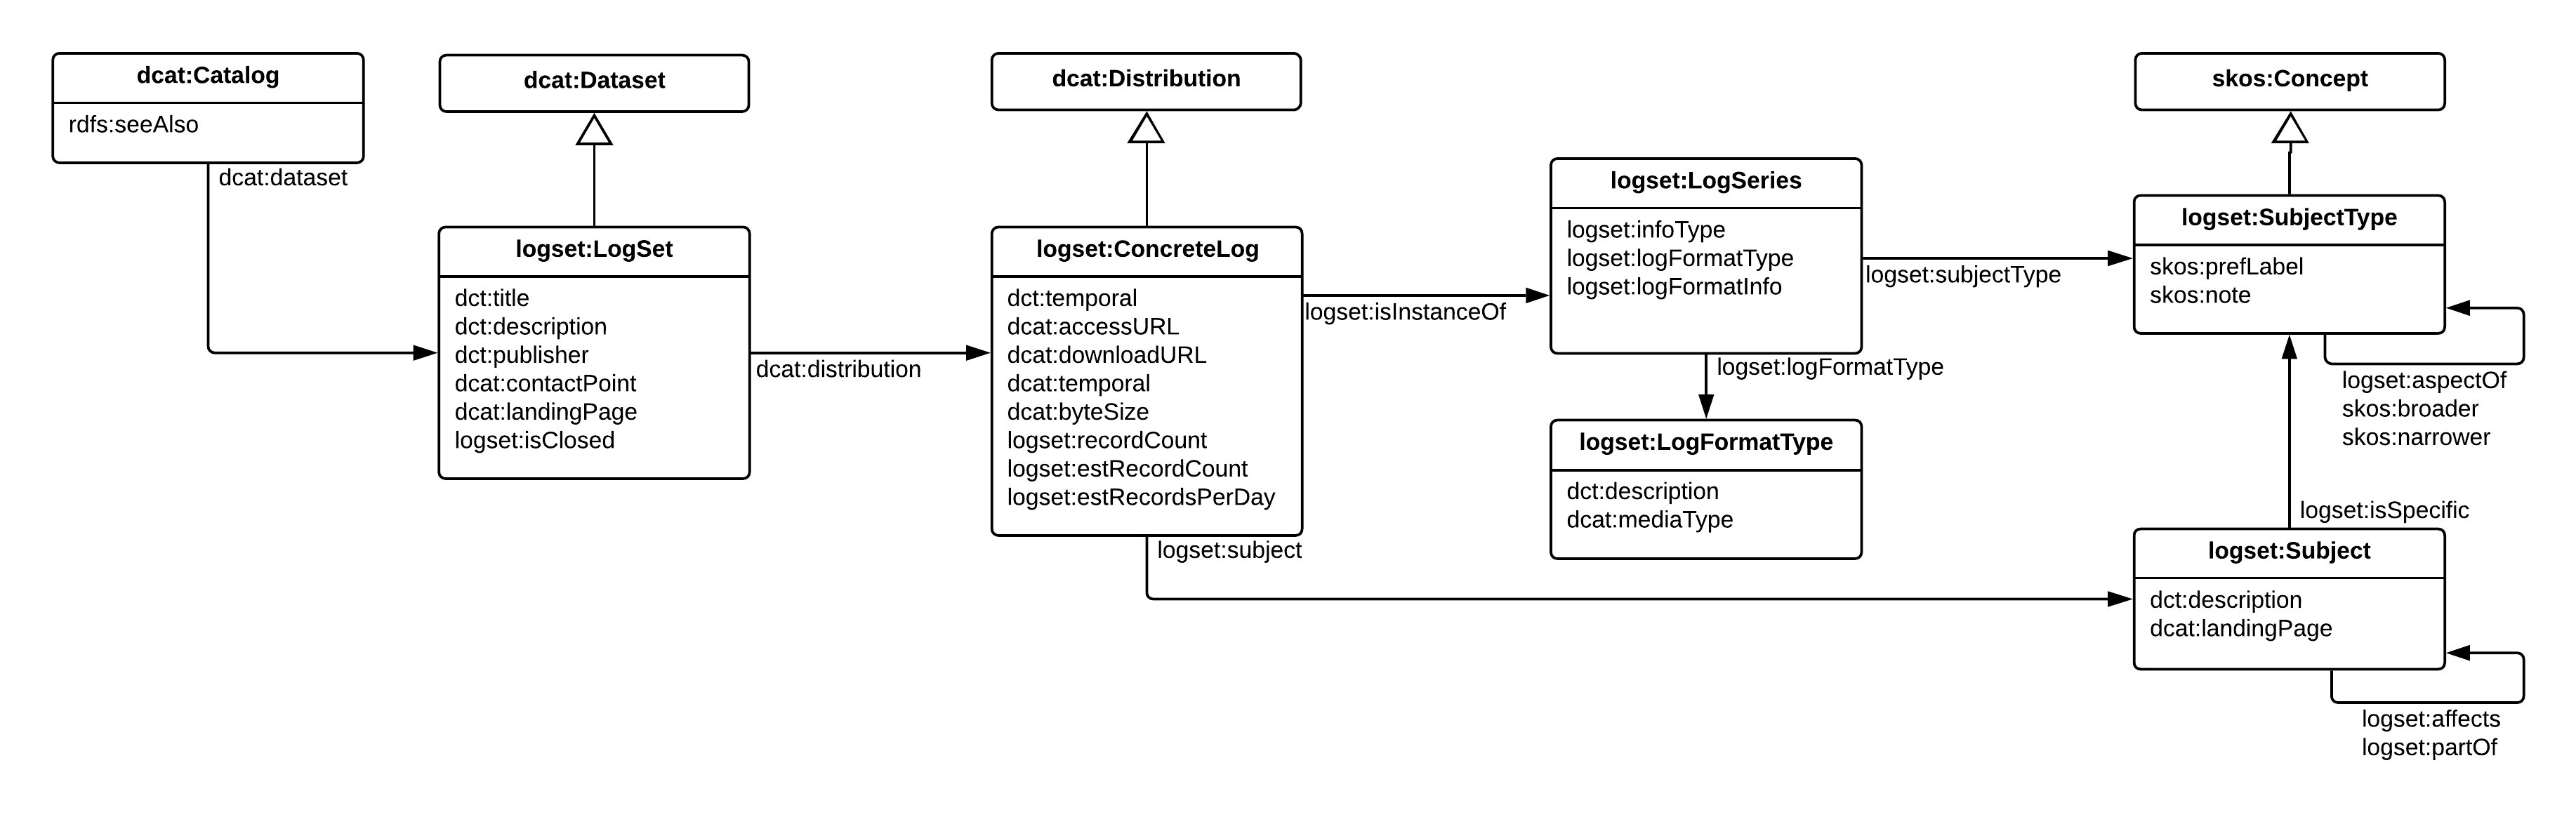
\includegraphics[width=0.9\textwidth]{logset-key-classes.png}
\caption{logset key classes}
\end{figure*}







